\subsection{Evaluating the coefficients in a 4D Gaussian mixture distribution}
\label{subsec: mixture}

The target $\pi$ is a mixture of $5$ Gaussian distributions on $\mathbb R^4$ with unequal weights, means $\vartheta_1, \dots, \vartheta_5$ near the vertices of a regular simplex of edge $4.5$, and covariance matrices of random orientation, so that $U = -\log \pi$ is not convex. The stochastic gradient $\nabla \hat U(x;\xi)$ adds to $\nabla U(x)$ either a Gaussian noise $\xi \sim \mathcal N(0, I_4)$, with $\mathcal C(x) = I_4$, or a non-Gaussian noise, a vector of independent centered exponential random variables of unit variance, rotated and scaled depending on $x$, with $\mathcal C(x) = \bigl( 2 - \pi(x)/\pi(\vartheta_1) \bigr)\, I_4$. Both covariances belong to the first row of Table~\ref{tab: explicit representors}, so the exact coefficients of the numerical bias follow from \eqref{eq: coefficients riesz} by quadrature. The test functions $f_1, \dots, f_4$, given in the panel titles of Figure~\ref{fig: bias gaussian} with vectors $a_1, a_2$ of lengths $1$, $0.6$ and the phase $\varphi_2$, have explicit expectations under $\pi$; they are taken from a pool of $12$, among the functions whose exact coefficients exceed $0.024$ in absolute value for both schemes and both noises.

\begin{figure}[htb]
\centering
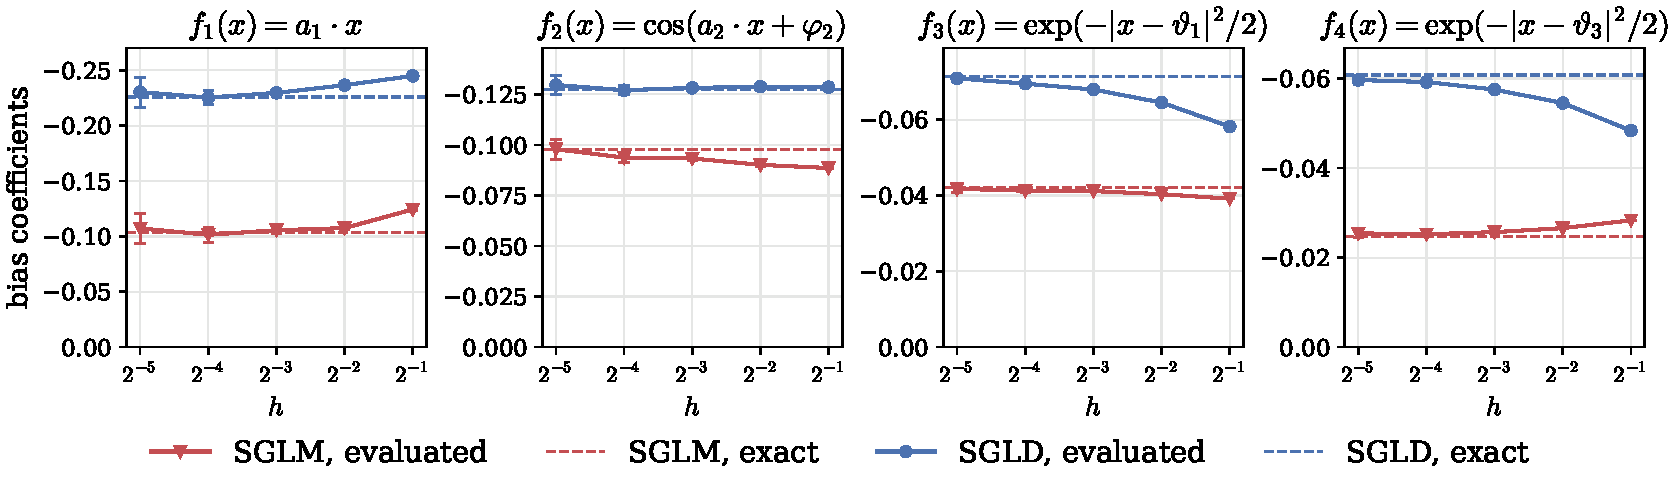
\includegraphics[width=0.96\textwidth]{figures/bias_gaussian.pdf}
\caption{Gaussian noise: the evaluated coefficients $(\pi_h(f) - \pi(f))/h$ of SGLM and $(\bar\pi_h(f) - \pi(f))/h$ of SGLD, with error bars of $2$ standard errors, and the exact coefficients \eqref{eq: coefficients riesz}, dashed. The vertical axis starts at $0$ and is reversed for negative exact coefficients.}
\label{fig: bias gaussian}
\end{figure}

\begin{figure}[htb]
\centering
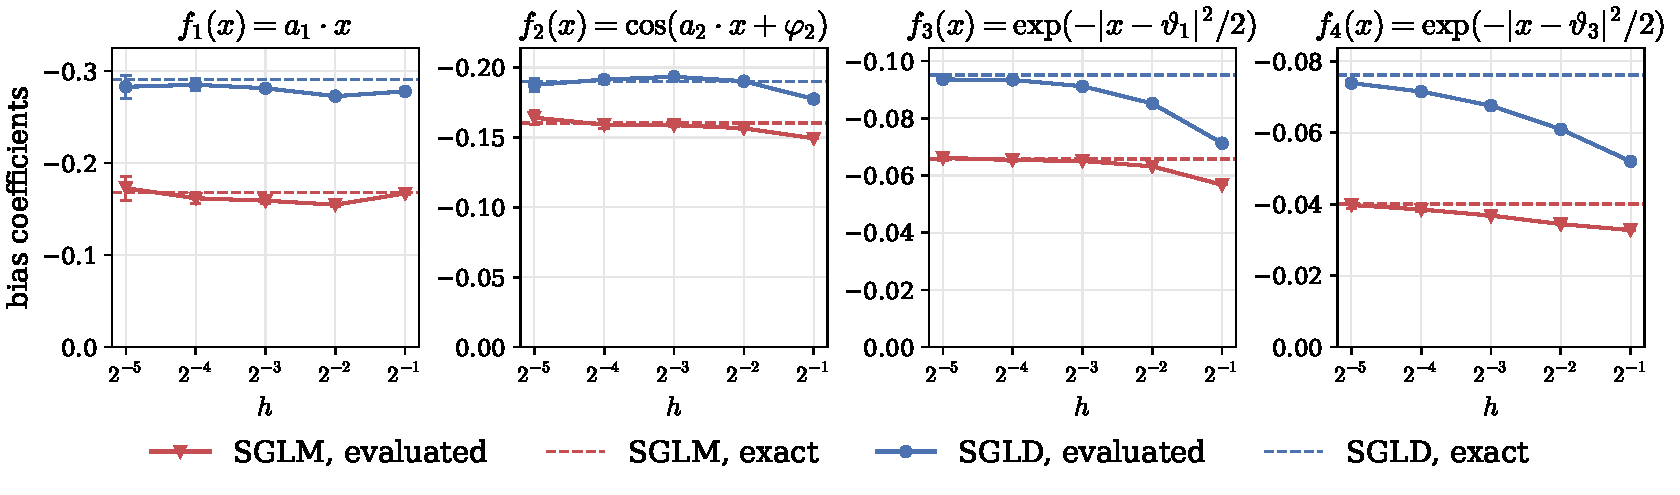
\includegraphics[width=0.96\textwidth]{figures/bias_nongaussian.pdf}
\caption{Non-Gaussian noise: the evaluated coefficients $(\pi_h(f) - \pi(f))/h$ of SGLM and $(\bar\pi_h(f) - \pi(f))/h$ of SGLD, with error bars of $2$ standard errors, and the exact coefficients \eqref{eq: coefficients riesz}, dashed. The vertical axis starts at $0$ and is reversed for negative exact coefficients.}
\label{fig: bias nongaussian}
\end{figure}

The evaluated coefficients $(\pi_h(f) - \pi(f))/h$ of SGLM and $(\bar\pi_h(f) - \pi(f))/h$ of SGLD are obtained from the time averages of $16$ chains, each over the time $5 \times 10^7$, at $h = 2^{-1}, \dots, 2^{-5}$. In Figures~\ref{fig: bias gaussian} and~\ref{fig: bias nongaussian}, they approach the exact coefficients as $h$ decreases, for every test function, both schemes and both noises; at $h = 2^{-5}$, the relative difference is at most $3.8\%$. The agreement under the non-Gaussian noise, whose third moments do not vanish, is in line with \eqref{eq: bias coefficient} and \eqref{eq: sgld coefficient}, in which the gradient noise enters only through its covariance $\mathcal C(x)$. For each of these test functions and both noises, the exact coefficient of SGLM is smaller in absolute value than that of SGLD, between $41\%$ and $84\%$ of it.

\begin{table}[htb]
\centering
\small
\begin{tabular}{llccccc}
\toprule
noise & integrator & $\frac12 \norm{\psi\,\pi}_{\mathrm{KR}}$ & $f_1$ & $f_2$ & $f_3$ & $f_4$ \\
\midrule
\multirow{2}{*}{Gaussian} & SGLM & $0.5643$ & $18.3\%$ & $28.9\%$ & $12.3\%$ & $7.2\%$ \\
 & SGLD & $0.9824$ & $23.0\%$ & $21.6\%$ & $12.0\%$ & $10.2\%$ \\
\midrule
\multirow{2}{*}{non-Gaussian} & SGLM & $0.9701$ & $17.4\%$ & $27.5\%$ & $11.2\%$ & $6.8\%$ \\
 & SGLD & $1.3636$ & $21.3\%$ & $23.2\%$ & $11.5\%$ & $9.2\%$ \\
\bottomrule
\end{tabular}
\caption{Exact coefficients $\frac12 \norm{\psi\,\pi}_{\mathrm{KR}}$ of the Wasserstein-1 errors in Corollary~\ref{cor: w1 limits}, with $\psi = \psi_{\mathcal C}$ for SGLM and $\psi = \psi_{\nabla^2 U} + \psi_{\mathcal C}$ for SGLD. For each test function $f$ of Figure~\ref{fig: bias gaussian}, the percentage in the table shows $|\pi(f\psi)| / \bigl( \norm{\nabla f}_\infty \norm{\psi\, \pi}_{\mathrm{KR}} \bigr) \Le 1$, which is the ratio of its exact coefficient of the numerical bias, normalized by $\norm{\nabla f}_\infty$, to the exact coefficient of the Wasserstein-1 error.}
\label{tab: w1 coefficients}
\end{table}

Table~\ref{tab: w1 coefficients} lists the exact coefficients of the Wasserstein-1 errors in Corollary~\ref{cor: w1 limits}, calculated as in Section~\ref{subsec: kr computation} and extrapolated from grids with $n = 25, 50, 100$. The exact coefficient of SGLM is $57\%$ of that of SGLD under the Gaussian noise and $71\%$ under the non-Gaussian noise, so \eqref{eq: w1 comparison} holds for both noises. The ratios in Table~\ref{tab: w1 coefficients} are at most $0.29$, so the Wasserstein-1 error, a supremum over all test functions $f$ with $\norm{\nabla f}_\infty \Le 1$, exceeds the numerical bias of each of these test functions, normalized by $\norm{\nabla f}_\infty$, by a factor larger than $3$.

\subsection{Convergence of Wasserstein-1 error in a radial distribution}
\label{subsec: radial}

For a radial potential $U(x) = u(|x|)$ and the gradient noise $\sigma \xi$ with $\xi \sim \mathcal N(0, I_d)$, the covariance is $\mathcal C(x) = \sigma^2 I_d$, so both integrators commute with rotations. Hence the distributions $\pi_h$, $\bar\pi_h$ and $\pi$ are rotation invariant, and the Wasserstein-1 distance between two of them is determined by their radial densities. The radial parts of \eqref{eq: sgld} and of the Markovian form \eqref{eq: sglm markov} are Markov chains on $[0, \infty)$, whose invariant distributions are computed by discretizing their stationarity equations, and the representors $\psi_{\mathcal C} = \sigma^2 \bigl( U - \pi(U) \bigr)$ and $\psi_{\nabla^2 U}$ of \eqref{eq: psi hessian} are radial, with $\norm{\psi\,\pi}_{\mathrm{KR}} = \int_0^\infty \bigl| \int_{|x| \Le r} \psi \, \D\pi \bigr| \, \D r$. The evaluated coefficients $\mathcal W_1(\pi_h, \pi)/h$ and $\mathcal W_1(\bar\pi_h, \pi)/h$ at a given $h$, and the exact coefficients $\frac12 \norm{\psi\,\pi}_{\mathrm{KR}}$ of Corollary~\ref{cor: w1 limits}, are thus computed without sampling in every dimension. The potential is
\begin{equation}
    u(r) = (r^2 - r)\, \frac{r^2}{r^2 + 1/4} ,
    \label{eq: radial potential}
\end{equation}
which grows quadratically and is not globally convex, with a ring of minima at $|x| \approx 0.64$. Since $u(r) = -4r^3 + \mathcal O(r^4)$ near $r = 0$, $U$ is not three times differentiable at the origin and does not satisfy Assumption~\ref{ass: U}; the example mainly serves to observe the convergence of the Wasserstein-1 error numerically.

\begin{figure}[htb]
\centering
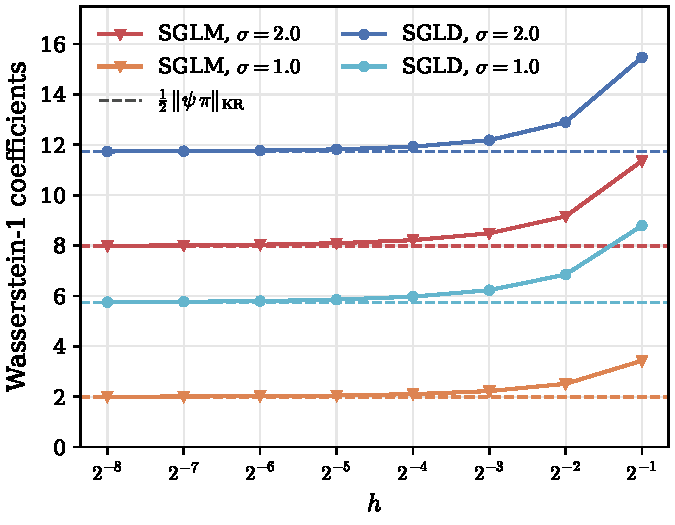
\includegraphics[width=0.46\textwidth]{figures/wasserstein.pdf}
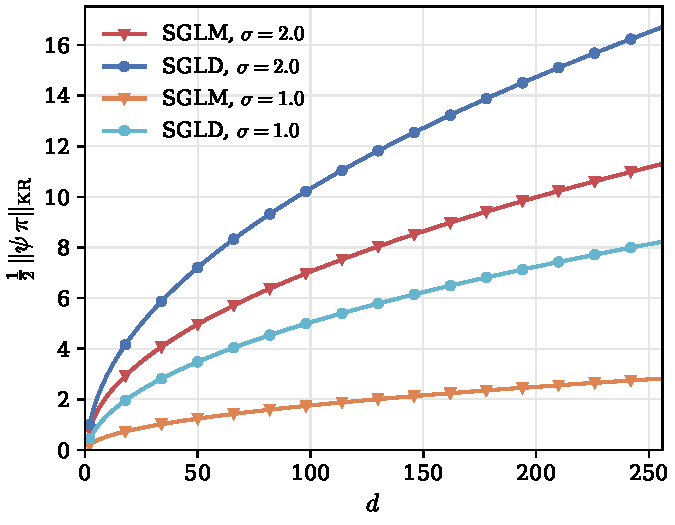
\includegraphics[width=0.46\textwidth]{figures/coefficients.pdf}
\caption{Radial potential \eqref{eq: radial potential} with the gradient noise $\sigma \xi$, $\xi \sim \mathcal N(0, I_d)$. Left: the evaluated coefficients $\mathcal W_1(\pi_h, \pi)/h$ of SGLM and $\mathcal W_1(\bar\pi_h, \pi)/h$ of SGLD in dimension $d = 128$, with the exact coefficients $\frac12 \norm{\psi\,\pi}_{\mathrm{KR}}$ of Corollary~\ref{cor: w1 limits}, dashed. Right: the exact coefficients against $d = 2, 4, \dots, 256$.}
\label{fig: radial}
\end{figure}

In Figure~\ref{fig: radial}, left, the evaluated coefficients converge to the exact coefficients for $\sigma = 1.0, 2.0$, and their distance to the exact coefficients halves with $h$; at $h = 2^{-8}$ it is between $0.09\%$ and $0.32\%$ of the exact coefficients. In this example the remainder of \eqref{eq: w1 limits} is therefore of order $h^2$, the order expected in Remark~\ref{rem: h2} under global strong convexity, although $U$ is not convex.

In Figure~\ref{fig: radial}, right, the exact coefficients grow like $\sqrt d$ for $d = 2, 4, \dots, 256$: from $d = 128$ to $d = 256$ with $\sigma = 1.0$, they are multiplied by $1.416$ for SGLM and by $1.434$ for SGLD, close to $\sqrt 2$. This is the growth in the Gaussian case $u(r) = r^2$, where both exact coefficients are proportional to $\mathbb E|X| \sim \sqrt d$ with $X \sim \mathcal N(0, I_d)$.

The exact coefficient of SGLM is below that of SGLD for every $d$ and both $\sigma$, so \eqref{eq: w1 comparison} holds throughout, and the advantage of SGLM is larger when the variance of the gradient noise is smaller: the ratio of the exact coefficient of SGLM to that of SGLD is $0.46$ at $d = 2$ and $0.34$ at $d = 256$ for $\sigma = 1.0$, against $0.81$ and $0.68$ for $\sigma = 2.0$. The exact coefficient of SGLM is proportional to $\sigma^2$, while that of SGLD contains the representor $\psi_{\nabla^2 U}$ of the discretization error of EM, which does not depend on $\sigma$.

\subsection{Bias correction of SGLM in a 16D product of ring distributions}
\label{subsec: rings}

The target $\pi$ on $\mathbb R^{16}$ is a product of $8$ ring distributions in rotated coordinates,
\begin{equation}
    U(x) = \sum_{i=1}^{8} u_i\Bigl( \sqrt{y_{2i-1}^2 + y_{2i}^2} \Bigr) , \qquad y = Q x , \qquad u_i(r) = \frac{r^2}{2} + \beta_i\, e^{-r^2/2} ,
    \label{eq: ring potential}
\end{equation}
with a random orthogonal matrix $Q$ and $\beta_1, \dots, \beta_8$ drawn uniformly from $[2, 4]$. Each $u_i$ has a ring of minima at $r = \sqrt{2 \log \beta_i}$, so $U$ is not convex. The gradient noise added to $\nabla U(x)$ is either a Gaussian one $\xi \sim \mathcal N(0, I_{16})$, or a non-Gaussian one: on each pair $(x_{2i-1}, x_{2i})$, a vector of $2$ independent centered exponential random variables of unit variance, rotated by the angle $x_{2i-1} + x_{2i}$. Both noises have the covariance $\mathcal C(x) = I_{16}$, so $\psi_{\mathcal C} = U - \pi(U)$ by the first row of Table~\ref{tab: explicit representors}. The third moments of the non-Gaussian noise do not vanish and depend on $x$.

SGLM is run at the step sizes $h = 2^{-4}$ and $2h = 2^{-3}$, with $32$ chains, each over the time $2 \times 10^7$, at each step size. The expectations $\pi_h(f)$ and $\pi_{2h}(f)$ are replaced by the time averages of $f$ over the chains. The means $\pi(f)$ and the exact coefficients $\frac12\, \pi(f \psi_{\mathcal C}) = \frac12 \bigl( \pi(fU) - \pi(f)\, \pi(U) \bigr)$ are each computed with $1.024 \times 10^{10}$ exact samples of $\pi$. The test functions for evaluating the numerical bias are chosen as
\begin{align*}
    f_1(x) &= x_1 , & f_2(x) &= \frac14 \sum_{j=1}^{16} x_j , \\
    f_3(x) &= \cos x_1 , & f_4(x) &= \sin(x_1 + x_2) , \\
    f_5(x) &= \sqrt{1 + x_1^2} , & f_6(x) &= e^{-(x_1^2 + x_2^2)/2} , \\
    f_7(x) &= \log\bigl( 1 + e^{x_1 - x_2} \bigr) , & f_8(x) &= \sqrt{1 + |x|^2} , \\
    f_9(x) &= \cos(x_1 + x_2) , & f_{10}(x) &= \sqrt{1 + x_1^2 + x_2^2} , \\
    f_{11}(x) &= \frac{x_1 x_2}{\sqrt{1 + x_1^2 + x_2^2}} , & f_{12}(x) &= \log\bigl( 1 + x_1^2 + x_2^2 + x_3^2 + x_4^2 \bigr) .
\end{align*}

For each test function, Tables~\ref{tab: bias correction gaussian} and~\ref{tab: bias correction nongaussian} list the approximations of $\pi(f)$ in Table~\ref{tab: approximations} at $h = 2^{-4}$, each with $\pi(f)$ subtracted, where $\varphi_{\mathcal C}$ of \eqref{eq: shift potential} is approximated by minimizing \eqref{eq: extrapolated energy}.

\begin{table}[htb]
\centering
\small
\begin{tabular}{ll}
\toprule
method & approximation of $\pi(f)$ \\
\midrule
SGLM & $\pi_h(f)$ \\
explicit coefficient & $\pi_h(f) - \frac h2\, \pi(f \psi_{\mathcal C})$ \\
extrapolation & $2\pi_h(f) - \pi_{2h}(f)$ \\
shifting correction & $\pi_h\bigl( f(x + h \nabla \varphi_{\mathcal C}(x)) \bigr)$ \\
\bottomrule
\end{tabular}
\caption{The approximations of $\pi(f)$ by SGLM and by the approaches of Section~\ref{sec: representors}, listed in the columns SGLM, explicit, extrapolation and shift of Tables~\ref{tab: bias correction gaussian} and~\ref{tab: bias correction nongaussian}.}
\label{tab: approximations}
\end{table}

The entry of SGLM is the numerical bias $\pi_h(f) - \pi(f)$, and the entries of explicit, extrapolation and shift are the errors of the approaches of Section~\ref{sec: representors}. The column explicit uses the exact coefficient, as in Section~\ref{subsec: explicit representors}, and the column extrapolation is the error bounded in \eqref{eq: extrapolation estimate}.

The column shift uses the postprocessed samples \eqref{eq: shifting correction}, with $\varphi_{\mathcal C}$ approximated by a neural network with $3$ hidden layers of width $64$, trained on $1.68 \times 10^7$ states of SGLM at each of the step sizes $h$ and $2h$, stored once per unit of time along $32$ chains and thus covering the total time $1.68 \times 10^7$. The change $\pi_h\bigl( f(x + h \nabla \varphi_{\mathcal C}(x)) \bigr) - \pi_h(f)$ is computed on states of runs at $h$ independent of the training states and added to the time average of $f$ at $h$.

\begin{table}[htb]
\centering
\small
\begin{tabular}{lcccc}
\toprule
 & SGLM & explicit & extrapolation & shift \\
\midrule
$f_{1}$ & $-8.64\times10^{-5}$ & $\boldsymbol{-8.57\times10^{-5}}$ & $-3.00\times10^{-4}$ & $-5.36\times10^{-4}$ \\
$f_{2}$ & $\boldsymbol{-1.83\times10^{-4}}$ & $-1.85\times10^{-4}$ & $-5.42\times10^{-4}$ & $-8.86\times10^{-4}$ \\
$f_{3}$ & $-4.86\times10^{-3}$ & $\boldsymbol{-6.73\times10^{-5}}$ & $1.49\times10^{-4}$ & $1.86\times10^{-4}$ \\
$f_{4}$ & $\boldsymbol{-2.63\times10^{-5}}$ & $-2.68\times10^{-5}$ & $-9.72\times10^{-5}$ & $-2.61\times10^{-4}$ \\
$f_{5}$ & $5.70\times10^{-3}$ & $\boldsymbol{1.08\times10^{-4}}$ & $-2.63\times10^{-4}$ & $-2.29\times10^{-4}$ \\
$f_{6}$ & $-2.99\times10^{-3}$ & $\boldsymbol{-1.51\times10^{-5}}$ & $4.67\times10^{-5}$ & $1.50\times10^{-4}$ \\
$f_{7}$ & $3.86\times10^{-3}$ & $6.38\times10^{-5}$ & $-2.60\times10^{-4}$ & $\boldsymbol{-1.71\times10^{-6}}$ \\
$f_{8}$ & $3.61\times10^{-2}$ & $\boldsymbol{5.07\times10^{-4}}$ & $-1.48\times10^{-3}$ & $-1.99\times10^{-3}$ \\
$f_{9}$ & $-3.97\times10^{-3}$ & $\boldsymbol{-2.48\times10^{-7}}$ & $2.29\times10^{-5}$ & $1.11\times10^{-4}$ \\
$f_{10}$ & $1.00\times10^{-2}$ & $\boldsymbol{1.59\times10^{-4}}$ & $-3.98\times10^{-4}$ & $-5.42\times10^{-4}$ \\
$f_{11}$ & $9.84\times10^{-5}$ & $\boldsymbol{-3.18\times10^{-5}}$ & $-1.08\times10^{-4}$ & $1.35\times10^{-4}$ \\
$f_{12}$ & $1.11\times10^{-2}$ & $\boldsymbol{1.19\times10^{-4}}$ & $-3.47\times10^{-4}$ & $-3.33\times10^{-4}$ \\
\bottomrule
\end{tabular}
\caption{Gaussian noise: the numerical bias $\pi_h(f) - \pi(f)$ of SGLM at $h = 2^{-4}$ and the errors of the explicit coefficient, the extrapolation and the shifting correction of Section~\ref{sec: representors}. The entry of smallest absolute value in each row is in bold.}
\label{tab: bias correction gaussian}
\end{table}

\begin{table}[htb]
\centering
\small
\begin{tabular}{lcccc}
\toprule
 & SGLM & explicit & extrapolation & shift \\
\midrule
$f_{1}$ & $\boldsymbol{1.99\times10^{-4}}$ & $2.00\times10^{-4}$ & $6.42\times10^{-4}$ & $2.44\times10^{-3}$ \\
$f_{2}$ & $5.56\times10^{-5}$ & $5.38\times10^{-5}$ & $\boldsymbol{-3.11\times10^{-5}}$ & $1.32\times10^{-3}$ \\
$f_{3}$ & $-4.76\times10^{-3}$ & $3.22\times10^{-5}$ & $\boldsymbol{4.79\times10^{-6}}$ & $3.09\times10^{-4}$ \\
$f_{4}$ & $\boldsymbol{4.94\times10^{-4}}$ & $\boldsymbol{4.94\times10^{-4}}$ & $-9.99\times10^{-4}$ & $5.61\times10^{-4}$ \\
$f_{5}$ & $5.63\times10^{-3}$ & $\boldsymbol{3.87\times10^{-5}}$ & $-1.91\times10^{-4}$ & $-4.42\times10^{-4}$ \\
$f_{6}$ & $-2.98\times10^{-3}$ & $\boldsymbol{-5.15\times10^{-6}}$ & $5.24\times10^{-5}$ & $7.70\times10^{-5}$ \\
$f_{7}$ & $4.02\times10^{-3}$ & $\boldsymbol{2.27\times10^{-4}}$ & $2.61\times10^{-4}$ & $1.13\times10^{-3}$ \\
$f_{8}$ & $3.61\times10^{-2}$ & $\boldsymbol{5.43\times10^{-4}}$ & $-1.44\times10^{-3}$ & $-1.76\times10^{-3}$ \\
$f_{9}$ & $-4.00\times10^{-3}$ & $\boldsymbol{-3.50\times10^{-5}}$ & $-8.72\times10^{-5}$ & $-1.78\times10^{-4}$ \\
$f_{10}$ & $1.00\times10^{-2}$ & $\boldsymbol{1.47\times10^{-4}}$ & $-4.08\times10^{-4}$ & $-3.72\times10^{-4}$ \\
$f_{11}$ & $2.07\times10^{-4}$ & $\boldsymbol{7.66\times10^{-5}}$ & $1.37\times10^{-4}$ & $3.47\times10^{-4}$ \\
$f_{12}$ & $1.11\times10^{-2}$ & $\boldsymbol{7.75\times10^{-5}}$ & $-4.24\times10^{-4}$ & $-6.31\times10^{-4}$ \\
\bottomrule
\end{tabular}
\caption{Non-Gaussian noise: the same quantities as in Table~\ref{tab: bias correction gaussian}, with the entry of smallest absolute value in each row in bold.}
\label{tab: bias correction nongaussian}
\end{table}

In general, the explicit coefficient has the smallest errors: it removes the term of order $h$ of the bias with the exact coefficient, and what remains is the remainder of \eqref{eq: kr sglm} and the fluctuation of the time averages. The extrapolation and the shifting correction have larger errors for some test functions, mainly from the additional error of the run at $2h = 2^{-3}$. Formally, the term of order $h^2$ of $\pi_{2h}(f) - \pi(f)$ is $4$ times that of $\pi_h(f) - \pi(f)$, so $2\pi_h(f) - \pi_{2h}(f) - \pi(f)$ carries the term of order $h^2$ of $\pi_h(f) - \pi(f)$ with the factor $-2$, against $1$ for the explicit coefficient; for $f_4$ under the non-Gaussian noise, Table~\ref{tab: bias correction nongaussian} gives $-9.99\times10^{-4}$ for the extrapolation against $4.94\times10^{-4}$ for the explicit coefficient. The shifting correction inherits the additional error of the run at $2h$, since the term of order $h$ of $\pi_h\bigl( f(x + h \nabla \varphi_{\mathcal C}(x)) \bigr) - \pi_h(f)$ is formally $h\, \pi_h(\nabla f \cdot \nabla \varphi_{\mathcal C}) = \pi_h(f) - \pi_{2h}(f)$ by the minimization of \eqref{eq: extrapolated energy}; the entries of shift for $f_8$, $f_{10}$ and $f_{12}$ have, in both tables, the sign and size of those of extrapolation. The largest error of the shifting correction, $2.44\times10^{-3}$ for $f_1$ under the non-Gaussian noise, comes from the fluctuation of the stored states on which $\varphi_{\mathcal C}$ is trained, which cover the total time $1.68 \times 10^7$, against $6.4 \times 10^8$ for the time averages: on the stored states, $(\pi_{2h}(f_1) - \pi_h(f_1))/h$ is $-3.70\times10^{-2}$, with the standard error $1.69\times10^{-2}$, against $-7.08\times10^{-3}$ from the time averages, and the change caused by the shift, $2.24\times10^{-3}$, is close to $-h$ times $-3.70\times10^{-2}$. Nevertheless, the largest absolute error over $f_1, \dots, f_{12}$ is $3.61\times10^{-2}$ for SGLM under both noises, against at most $5.43\times10^{-4}$, $1.48\times10^{-3}$ and $2.44\times10^{-3}$ for the explicit coefficient, the extrapolation and the shifting correction; the corrections reduce the largest absolute error of SGLM by factors between $14.8$ and $71.1$, so the bias correction works in this example.
